\documentclass[border=5pt]{standalone}
\usepackage{tikz}
\usepackage{amsmath}

\begin{document}

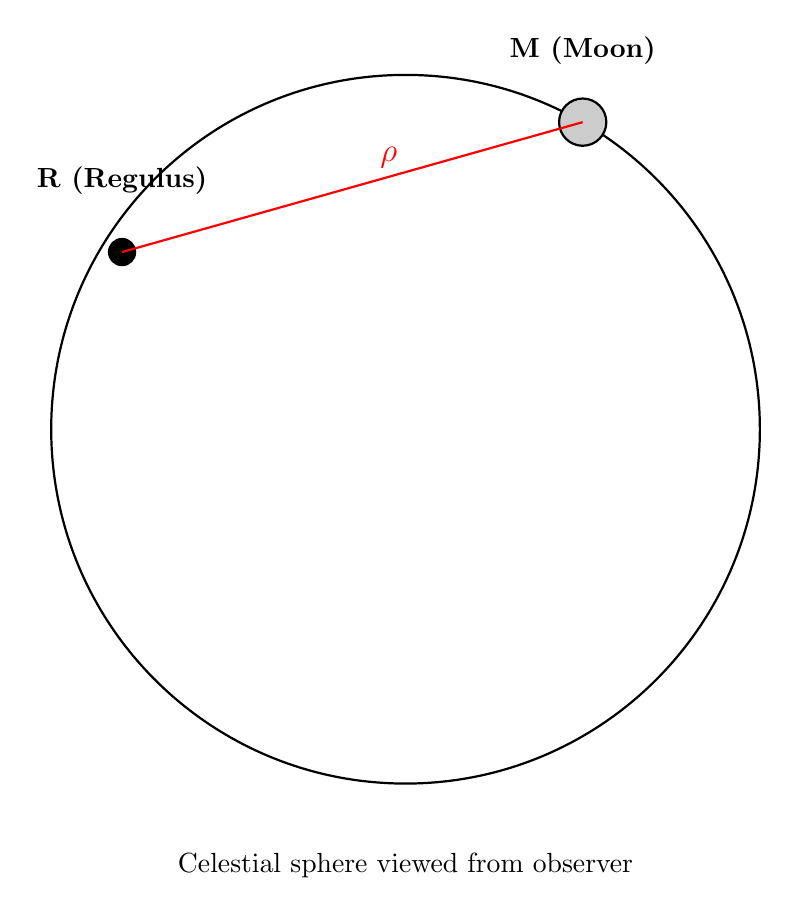
\begin{tikzpicture}[scale=1.5, thick]
  % Draw celestial sphere
  \draw (0,0) circle (3);
  
  % Moon position and label
  \fill[fill=gray!40] (1.5, 2.6) circle (0.2);
  \draw (1.5, 2.6) circle (0.2);
  \node[anchor=south] at (1.5, 3.0) {\textbf{M (Moon)}};
  
  % Star position and label
  \fill[fill=black] (-2.4, 1.5) circle (0.12);
  \node[anchor=south] at (-2.4, 1.9) {\textbf{R (Regulus)}};
  
  % Arc showing lunar distance
  \draw[thick, red] (1.5, 2.6) -- (-2.4, 1.5);
  \node[anchor=west, color=red, font=\large\bfseries] at (-0.3, 2.3) {$\rho$};
  
  % Greenwich reference
  \node[anchor=north] at (0, -3.5) {Celestial sphere viewed from observer};
\end{tikzpicture}

\end{document}
